\documentclass[a4paper,12pt]{article}
\usepackage{listings}
\usepackage{geometry}                % See geometry.pdf to learn the layout options. There are lots.
\geometry{a4paper}                   % \dots or a4paper or a5paper or \dots 
%\geometry{landscape}                % Activate for for rotated page geometry
\usepackage[parfill]{parskip}    % Activate to begin paragraphs with an empty line rather than an indent
\usepackage{graphicx}
\usepackage{amssymb}
\usepackage{epstopdf}
\usepackage{caption}
\usepackage{color}
\usepackage{url}
%\usepackage{helvet} %To the untrained eye helvetica and arial are pretty much identical
%\renewcommand{\familydefault}{\sfdefault}
\usepackage[utf8x]{inputenc}
\usepackage{tikz}
\usetikzlibrary{arrows}
\usetikzlibrary{calc}
\usepackage{color}
\usepackage{algpseudocode}
\usepackage{algorithm}
\usepackage{algorithmicx}
\usepackage{amsmath}
\tikzstyle{block} = [draw,fill=blue!20,minimum size=2em]
\tikzstyle{p} = [draw,fill=green!20,minimum size=2em]
\tikzstyle{h} = [draw,fill=yellow!20,minimum size=2em]
\tikzstyle{msg} = [draw,fill=orange!20,minimum size=2em]
\tikzstyle{final} = [draw,fill=green!20,minimum size=2em]
\tikzstyle{circle} = [draw,shape=circle,fill=red!20,minimum size=2em]
\tikzstyle{branch}=[fill,shape=circle,minimum size=3pt,inner sep=0pt]
\newcommand{\hash}[1]{\ensuremath{H(#1)}}
\newcommand{\Pad}{\text{Pad}}
\newcommand{\HF}{HF}
%opening
\title{Cracking Hasing Functions}
\author{Toby Gilham, Jonathan Poulter and Alan Saul}
\date{}

\begin{document}

\maketitle

%\section{Properties of a hashing function}

%it is easy to compute the hash value for any given message
%it is infeasible to generate a message that has a given hash
%it is infeasible to modify a message without changing the hash
%it is infeasible to find two different messages with the same hash
%\cite{http://tools.ietf.org/html/rfc4270}
%MD5 First announced in 1991

\section{Hashing a message}
Hashing functions are able to take a variable length message and from it create a fixed length output. A hashing function will always hash the same input to the same output. The special type of hashing functions, discussed here are cryptographic hashing functions, these have additional properties which mean they are used in a range of security applications.

A hashing function is a mapping for a binary string, $H$: $\{0,1\}^* \rightarrow \{0,1\}^n$, to create a fixed length digest. The number of distinct possible outputs of a hashing function of fixed length $L$ is $2^L$ theoretical digests. There are clearly vastly more valid inputs as the input may be of an arbitrary length, therefore there are necessarily collisions, due to the pigeon-hole effect. It is important however that there is no determinable connection between the message, $m$, and the digest, $H(m)$. $H$ should generate sufficiently random digests such that it fulfills three criteria:
\begin{itemize}
  \item it should be computationally infeasible to find some $m_1$ and $m_2$ where $m_1 \neq m_2$ and $H(m_1) = H(m_2)$, this is the \textbf{collision-free property}. This property is desirable because of hashes being used to distinguish input data. Collisions reduce the condifence one can have in a function for its ability to distinguish distinct inputs.
  \item given a digest $h$, it should be computationally infeasible to find any $m$ where $h = H(m)$. This is \textbf{first pre-image resistance}, this ensures it is difficult to retrieve a hashed message.
  \item  an input $m_1$, and the digest $H(m_1)$ it should be computationally infeasible to find a second message $m_2$ where $m_1 \neq m_2$ and $H(m_1) = H(m_2)$, this is \textbf{second pre-image resistance}. When a message and hash are found, it should be infeasible to find more messages which hash to the same value.
\end{itemize}

A tasking being computationally infeasibile refers to an adversary being unable to perform the action in a reasonable amount of time with reasonable resources.

\label{sec:propeties_of_a_hash}

\paragraph{The Random Oracle} An ideal fixed-length hashing function will play the role of a Random Oracle which  acts as a theoretically optimal cryptographic primitive. A Random Oracle, for a given input, produces a truly random output and the input and corresponding output are recorded. If the same input message is presented to the oracle at a later point the previously generated value is returned, however for each novel input presented a new random corresponding output will be generated.\\



There are many cryptographic hash functions, many vary in success at fulfilling the properties described. Yet they are integral cryptographic primitives on which many secure protocols are built. Successful cryptographic functions have many uses. In most operating systems user passwords are not stored in plain text, doing so would allow a user who maliciously gained access to the password store to know a user's password. Instead password hashes are stored and on login a user submits the password, which is hashed and verified against the stored hash, if these match then the user is authorised. Hashes are used for the signing digital documents and distinguishing large files without having to do explicit bit-wise comparison between each file, this method provides a method of verifying another's copy of a file and is able to identify matches or inconsistencies.

\section{The Merkle-Damg\r{a}rd Construction}
Various constructs can build a hashing function, however the most popular over the last two decades, which is the construction underlying the most dominant hashes in use today, is the Merkle-Damg\r{a}rd (MD) construction \cite{Merkle1979}.
The aim is to build a hashing function $H$ which takes an abitrary length message to create a digest, $\{0,1\}^* \xrightarrow{H} \{0,1\}^n$ in the same fashion as a random oracle would. In practice creating a straight-forward hashing or block cipher to take arbitrary input is impractical, most modern hashing functions, take some compression-function and repeatedly apply it to successive blocks of the message.

If a compression function $f$ is suitably provably random then it is possible to create a equally provably random $H$ by using the MD construction. The function takes a message an splits it into blocks of equal length therefore the construct only works on messages which have length, $L$ where $$L \equiv 0 \text{ (mod } n).$$

\subsection{MD-Compliant padding}
It is therefore necessary to apply padding to the original message. In the initial proposal Merkle simply padded the message with zeros\cite{Merkle1979}. This is sufficient to keep the important property of the construct, if $f$ is collision resistant, so is $H$, but more generally MD-compliant padding follows the following three rules. For messages $m$, $m_1$ and $m_2$ in the possible message space.
\begin{itemize}
    \item $m$ must be a prefix of $\Pad(m)$.\\\emph{The padding must be applied to the end of the message.}
    \item \textbf{if} $|m_1| = |m_2|$ \textbf{then} $|\Pad(m_1)| = |\Pad(m_2)|$.\\\emph{Two messages of the same length should pad to equal lengths also.}
    \item \textbf{if} $|m_1| \neq |m_2|$ \textbf{then} last block of $\Pad(m_1) \neq$ last block of $\Pad(m_1)$.\\\emph{This is to prevent a very simple suffix collisions, demonstrated in section \ref{sec:md5pad}.}
\end{itemize}

\subsection{The General Hashing Function}
Algorithm \ref{alg:hashing} shows the basic form of the MD construction. Though many modern hashing algorithms are based on the MD principle, including the SHA series \cite{fips} of hashes, these often make changes to the construct to side-step specific vulnerabilities in the original design. Here $f$ can be any collision-resistant compression function which will take an initialising vector and the current message block, $b_i$ and produce a new IV vector for the construct on each iteration of the loop, a collision-resistant hashing function. Figure \ref{fig:mdpic} illustrates the blocking of the original message, the presence of the padding element and the processing of the IVs.

\begin{algorithm}
    \caption{The Merkle-Damg\r{a}rd construction}
    \label{alg:hashing}
\begin{algorithmic}
    \Function{H}{$b_1$, \ldots, $b_l$}
        \State $y \gets IV_0$  
        \Comment{$IV_0$ is some initialising vector}
        \For{$i = 1 \rightarrow l$}
            \State $y \gets f(y, b_i)$
        \EndFor
        \State \Return $y$
    \EndFunction
\end{algorithmic}
\end{algorithm}



\begin{figure}
    \begin{center}
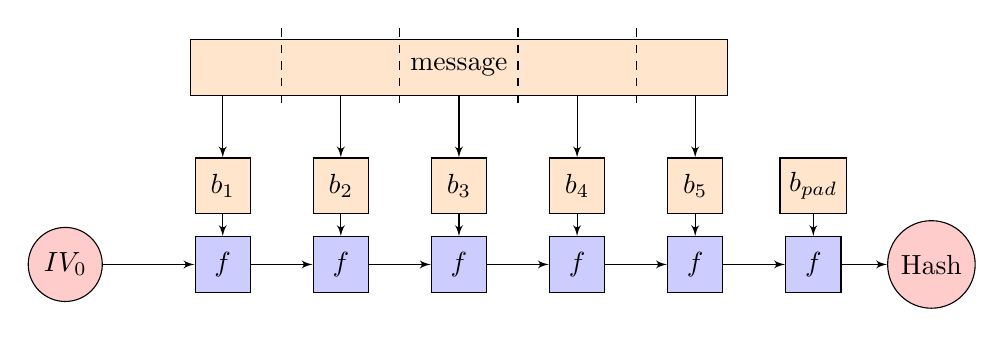
\begin{tikzpicture}[>=latex']

% Draw blocks, inputs and outputs
    \def\sp{1.5}
    \node[circle] at (1, -1) (IV) {$IV_0$};
    \node[msg, align = center, text width=12.5*\sp em] at (4*\sp, 1.5) (orig) {message};
    \foreach \y in {1,2,3,4,5} {
        \node[msg] at (\sp + \y*\sp,0) (input\y) {$b_\y$};
        \node[block] at (\sp+\y*\sp,-1) (block\y) {$f$};
        \draw[->] (input\y) -- (block\y);
        \pgfmathtruncatemacro{\n}{\y + 1}
        \draw[->]  (orig.south -| input\y) -- (input\y);
    }
    \foreach \y in {1,2,3,4} {
        \coordinate (x) at ($(input\y)+(0.75,1)$);
        \coordinate (y) at ($(x) + (0,1)$);
        \draw[dashed]  (y) -- (x) ;
    }
    \node[msg] at (7*\sp, 0) (pad) {$b_{pad}$};
    \node[block] at (7*\sp, -1) (final) {$f$};
    \node[circle] at (8*\sp, -1) (hash) {Hash};
    
    % join up
    \draw[->] (IV) -- (block1);
    \draw[->] (block5) -- (final);
    \draw[->] (final) -- (hash);
    \draw[->] (pad) -- (final);
    \foreach \y in {1,2,3,4} {
        \pgfmathtruncatemacro{\n}{\y + 1}
        \draw[->] (block\y.east) -- (block\n);
    }
    %\node[block] at (2,-6) (block6) {$f_6$};
    %\draw[->] (block6.east) -- +(0.5,0);


\end{tikzpicture}
\end{center}
\caption{The Merkle-Damg\r{a}rd construction: firstly the message is split into many blocks, each is sequentially processed by a compression function $f$ with some initial IV, $IV_0$, this produces new IV values, which are passed the the next usage of $f$. Finally the IVs are finalised using the MD padding block and the resulting IV is the given hash}
\label{fig:mdpic}
\end{figure}

\subsection{Weaknesses of the MD Construction}
As cryptanalysis has progressed the number of attacks on the MD construction itself has increased\cite{dobbertin}\cite{Xie2013}. It is important to note that these are not attacks on the specific compression functions used, though these also exist, but these attacks are directly against the MD structure and therefore would reduce the work needed to find collisions even using a perfect random-oracle for the compression function.

\subsection{Length-Extension Attack}
The first weakness of the simple MD construction is that once a single collision has been found it is trivial to find more\cite{Sasaki2006}. 

Let $H: \{0,1\}^* \rightarrow \{0,1\}^n$ be a hashing function and two distinct messages $m_1$ and $m_2$ are a collision pair, that is $H(m_1) = H(m_2)$, under the simple MD construction it is trivial to generate more collisions by appending the collision-causing message with a common message $x$ producing $H(m_1||x)$, $H(m_2||x)$.  Where $||$ is the concatenation operator.
{\color{red} another attack}



\label{sec:length}

\section{The MD5 Hashing Function}
The MD5 hashing algorithm\cite{Rivest} created in 1992 is an MD based hashing function. It has been widely used across the internet to store password hashes and is still dominant in providing file checksums, even though it has been shown to be collision weak MD5 is till commonly used in many situations. In the following section the algorithm itself is described as per the specification laid out in RFC 1321 \cite{Rivest}. A clear python implementation is included at the end of this report, the intention is to demonstrate a simple implementation which is useful for education rather than speed of execution.

\subsection{MD5 message preparation}
The MD5 digest algorithm processes a $b$-bit original message.
\paragraph{Padding}
\label{sec:md5pad}
A mandatory ``1'' bit is added to the end of the bit-string 
Padding ``0'' bits are added to the message to make the length, l, $$l \equiv 448 \text{ (mod } 512).$$

\paragraph{Length appending}
The message will be processed in blocks of 128-bits, to create a 128-bit ouput so the message length must be a multiple of 128-bit also. Also it is desirable to include the length-strengthening discussed in \ref{sec:length}. This has the ability to prevent some attacks, which the MD construction is weak against. So the bit-string is appended with the 64-bit representation of the number $b$. Now, $$l \equiv 0 \text{ (mod } 512).$$

\paragraph{IV intialisation}
Once the message has been prepared the MD construction is initialised, the intial vector of the construct ($IV_0$) is

\begin{tabular}{ l l l l}
	$A_0$ = \texttt{0x67452301}& $B_0$ = \texttt{0xefcdab89}& $C_0$ = \texttt{0x98badcfe}& $D_0$ = \texttt{0x10325476}
\end{tabular}

\subsection{The MD5 Compression Function}
Once the message has been prepared the MD5 compression function is ran over the padded message, 128-bits at a time. The compression function is illustrated in figure \ref{fig:md5comp} and is initliased to some given some IV, shown by $A, B, C, D$. $A$, from the IV is permuted by the function and the result is stored into the location of $B$. Firstly a non-linear combination of $B, C$ and $D$ is added, then the 32-bit block under consideration in the operation is added. A constant, derived from the mathematical $\sin$ function is added. $A$ is then subject to a left-bit rotation, by a varying number of places and then the contents of $B$ is also added. 64 variants of this operation are performed, they are grouped into blocks of 16, producing 4 `rounds'. It is important to note that all addition is modulo $2^{32}$, 32-bit addition.
The resulting hash is the concatenation of the IV components, $A || B || C || D$.
\begin{figure}
    \centering
    \includegraphics[width=0.5\textwidth]{md5.png}
    \caption{The MD5 compression function.}
    \label{fig:md5comp}
\end{figure}

\section{Attacking MD5}
An attack on a hacking function attempts to circumvent the secure properties that a hashed message should have: the one-way property and the collision-free property, discussed in section \ref{sec:propeties_of_a_hash}.
A first pre-image attack focuses on finding a message which has a particular hash-value, therefore circumventing the one-way property and tries to find $m$ where $\hash{m}$ is known. A further attack, a \emph{second-preimage} attack, where the original message $m_1$ is known, attempts to find another message $m_2$ where $\hash{m_1} = \hash{m_2}$.
A collision attack attempts to find any two arbitrary messages $m_1$ and $m_2$, where $\hash{m_1} = \hash{m_2}$.

\subsection{Collision Attacks}
Hoffman,of the Network Working Group, in 2004 discussed that the dominant hashing attacks are collision attacks. Considering the `birthday problem' it is possible to estimate how many evaluations of the hash function it would take to find a collision in a given hashing function. Given a message space of  $2^n$, where $n = 128$ for MD5, the `birthday bound' for a binary string is $2^{(n/2)}$; $2^{64}$ for MD5. This is a theoretical bound on finding a collision in a random oracle. In practice this is reliant on the `perfection' of the hashing function, that is that each possible 128-bit output should be equally likely and there should be no inferable connection between input and output. 

MD5 is not a perfect hashing function and many collisions have now been found, the first publicly announced collision was from Dobbertin in 1996 \cite{dobbertin}. The MD5 function processes the message to be digested into 64-byte chunks (blocks) and the collision detailed by Dobbertin relies on using previous blocks to put initialisation vectors of the MD construction into a specific state, from this state their are two distinct blocks which are able to cause a collision. This is not considered to be an attack on the full MD5 function; as a single message isn’t presented which causes a collision, but from 1996 the MD5 construction has been widely considered `broken’ with respect to being collision-resistant.

\begin{figure}
\begin{tabular}{|r|  l l l l|}
	$IV_0'$ :& $A_0'$ = \texttt{0x12AC2375}& $B_0'$ = \texttt{0x3B341042}& $C_0'$ = \texttt{0x5F62B97C}& $D_0'$ = \texttt{0x4BA763ED}\\& & & &\\
	$m_1$:& $X_0$ = \texttt{0xAA1DDa5E} & $X_4$ = \texttt{0x1006363E} & $X_8$ = \texttt{0x98A1FB19} & $X_{12}$ = \texttt{0x1326ED65} \\
	& $X_1$ = \texttt{0xD97ABFF5} & $X_5$ = \texttt{0x7218209D} & $X_9$ = \texttt{0x1FAE44B0} & $X_{13}$ = \texttt{0xD93E0972} \\
	& $X_2$ = \texttt{0x55F0E1C1} & $X_6$ = \texttt{0xE01C135D} & $X_{10}$ = \texttt{0x236BB992} & $X_{14}$ = \texttt{0xD458C868} \\
	& $X_3$ = \texttt{0x32774244} & $X_7$ = \texttt{0x9DA64D0E} & $X_{11}$ = \texttt{0x6B7A669B} & $X_{15}$ = \texttt{0x6B72746A} \\
	$m_2$: & \multicolumn{4}{c|}{$m1$ with the following change $m_2[X_{14}] = m_1[X_{14}] + 2^9$ }\\& & & &\\
	MD5: & \multicolumn{4}{l|}{\texttt{0xBF90E670 0x752AF92B 0x9CE4E3E1 0xB12CF8DE}}
\end{tabular}
\caption{The collision demonstrated by Dobbertin\cite{dobbertin}. This demonstrates a ``collision of the compress function'' and not on the full hash itself as it relies on getting the algorithm into a point of using these IVs.}
\label{fig:coldob}

\end{figure}

There have been many distributed projects which have tasked themselves with finding MD5 collisions on the full algorithm and the first of these to report results was MD5CRK\cite{Wang2004}. This project yielded two full colliding message pairs for the MD5 algorithm, one is shown in figure \ref{fig:coldob}. Collisions were also presented for the MD4, RIPEMD and HAVAL-128 protocols. Each message presented for MD5 was made of two blocks, each first block was identical and had the effect of forcing the MD construction into using a fixed IV while processing the second block which can be given two distinct blocks and still produce the same hash. The MD5CRK algorithm spent the majority of its time finding a block which is able to generate an exploitable IV, after this is found it took very little time to produce a second block which is able to break collision-resistance.

%{\color{red}
%Tunneling

%The  \cite{Klima2006} presented tunnelling 
%}

The same group, 6 years later presented the first public MD5 collision using a single block \cite{Xie2013}, this collision is shown in figure \ref{fig:colxie}. The implocation of being able to generate these collisions easily has already been exploited, most notoriously in the production of fake signed website certificates \cite{Stevens}, as this becomes more feasible and computational tractable the chance of generating even more `useful' collisions increases. A useful collision is not only a collision in the compression function, but a collision which can be used for some form of gain.
\begin{figure}
\begin{tabular}{|r|  l l l l|}
$M_0$:& $X_0$ = \texttt{0x6165300E} & $X_4$ = \texttt{0x6503CF04} & $X_8$ = \texttt{0x2F94CC40} & $X_{12}$ = \texttt{0x6D658673} \\
	& $X_1$ = \texttt{0x87A79A55} & $X_5$ = \texttt{0x854F709E} & $X_9$ = \texttt{0x15A12DEB} & $X_{13}$ = \texttt{0xA4341F7D} \\
	& $X_2$ = \texttt{0xF7C60BD0} & $X_6$ = \texttt{0xFB0FC034} & $X_{10}$ = \texttt{0x5C15F4A3} & $X_{14}$ = \texttt{0x8FD75920} \\
	& $X_3$ = \texttt{0x34FEBD0B} & $X_7$ = \texttt{0x874C9C65} & $X_{11}$ = \texttt{0x490786BB} & $X_{15}$ = \texttt{0xEFD19d5A} \\
$M_1$:& $X_0$ = \texttt{0x6165300E} & $X_4$ = \texttt{0x6503CF04} & $X_8$ = \texttt{0x2F94CC40} & $X_{12}$ = \texttt{0x6D658673} \\
& $X_1$ = \texttt{0x87A79A55} & $X_5$ = \texttt{0x854F7{\underline 4}9E} & $X_9$ = \texttt{0x15A12DEB} & $X_{13}$ = \texttt{0xA4341F7D} \\
    & $X_2$ = \texttt{0xF7C60BD0} & $X_6$ = \texttt{0xFB0FC034} & $X_{10}$ = \texttt{0x{\underline D}C15F4A3} & $X_{14}$ = \texttt{0x8FD75920} \\
	& $X_3$ = \texttt{0x34FEBD0B} & $X_7$ = \texttt{0x874C9C65} & $X_{11}$ = \texttt{0x490786BB} & $X_{15}$ = \texttt{0xEFD19d5A} \\
    MD5: & \multicolumn{4}{l|}{\texttt{0xF999C8CA 0xF7939AB6 0x84F3C481 0x1457CB23}}
%0x6165300e,0x87a79a55,0xf7c60bd0,0x34febd0b,0x6503cf04,0x854f749e,0xfb0fc034,0x874c9c65, 0x2f94cc40,0x15a12deb,0xdc15f4a3,0x490786bb,0x6d658673,0xa4341f7d,0x8fd75920,0xefd18d5a

\end{tabular}
\caption{The single-block collision demonstrated by Xie\cite{Xie2013}. Modified bits are underlined, this entire collision actually only differs by two bits.\\$0 \rightarrow 4$: \texttt{0000} $\rightarrow$ \texttt{0100} and 
$5 \rightarrow D$: \texttt{1101} $\rightarrow$ \texttt{0101}.
}
\label{fig:colxie}
\end{figure}

%{\color{red}

%Implications of quickly being able to identify MD5 collisions.

%What existing uses of MD5 would be broken. What would a malicious user be able to do?
%What would we use instead of MD5?
%Why would it be better? -> bigger output domain $2^128$ for MD5, $2^512$ for SHA-2.
%Better S-box (catchy name for the compression function (I think)) http://upload.wikimedia.org/wikipedia/commons/thumb/7/7d/SHA-2.svg/400px-SHA-2.svg.png

%}

\subsection{Pre-image attacks}
Producing and publishing a collision, may not present a security problem for many uses of hashes, producing a collision for a hashed password may be enough to enter a single system but doesn't necessarily give the attacker the plaintext password. The hashed information is still safe. Once victim to collision attacks most cryptographers will avoid a hash\cite{Stevens}, yet more crippling to the reputation of the hashing function is a pre-image attack.

For a given $H$: $\{0,1\}^* \rightarrow \{0,1\}^n$ a pre-image attack on a hash, $h$, is able to retrieve $m$ where $h = H(m)$. For an ideal $H$ (which strictly models a Random Oracle) a brute-force attack is necessary, for MD5 this should take $2^{128}$ evaluations of the MD5 function for an arbitrary $m$.

Performing pre-image attacks on arbitrary hashes is clearly a time-consuming task it is therefore desirable to perform some pre-computation to make performing multiple attacks faster, this time-memory tradeoff attempts to save chains of hashes which cover all of a sub-space of the entire message-space. 

For a hash $H$: $\{0,1\}^* \rightarrow \{0,1\}^n$ and a finite password set $P$; one example might be alpha-numeric strings less than 9 characters in length. The perfect data-structure is, for each password in $P$ store $p$ and $H(p)$, this is infeasible and would require storage $\text{O}(|P| \times n)$ bits of storage.

\paragraph{Hash chain tables}
Instead a reduction function $R$ is produced to take a hash and produce a new message from it, where $h \in H$ and $p \in P$. $R$ produces the mapping $h \rightarrow p$, this allows for an alternating chain of \emph{message to hash to message\dots} to be produced.

To generate a hash-chain table\cite{Hellman1980}, a random set of passwords from P is selected. Each of these is hashed, then the resulting hash is gien to the reduction function, this is then hashed, this process is repeated $k$ times, where $k$ is the chain length. Instead of storing the entire chain, simply the starting point and the last password are stored. 
\begin{center}
    password $\xrightarrow{H}$ \textsc{2867c6a4} $\xrightarrow{R}$ tadcaacc $\cdots$ nomzyaw$\xrightarrow{H}$ 3b5440e1 $\xrightarrow{R}$ bffbbecf
\end{center}
Here only `password' and `bffbbecf' need to be stored to retrace every hash, and thefore generating password, seen while creating the table.

To use the table to attack a hash $h$, firstly the hash is passed through the reduction function, to produce a candidate password $p$. If this $p$ appears in the set of endpoints of the table then the corresponding starting password is selected and the series of hash-reductions is applied until the original $h$ is seen, the $p$ which generated $h$ is the plaintext preceding $h$ in the chain. 
It isn't guaranteed that this search will be successful as multiple hashes are likely to reduce to the same $p$, this is illustrated in figure \ref{fig:table}. If unsuccessful further hash-reducing is performed on $h$ until a chain of length $k$ is reached. If the hash is not discovered before reaching $k$, then the hash was never seen during the creation of the table and the search has failed.
\begin{figure}
    \begin{center}
    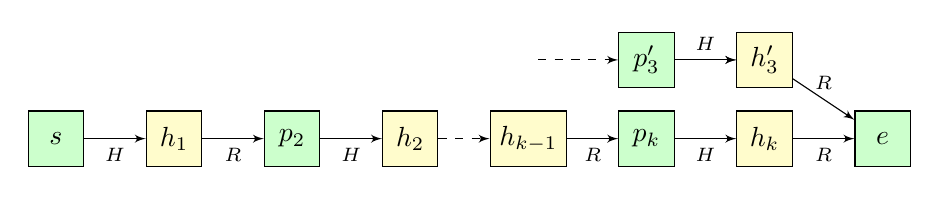
\begin{tikzpicture}[>=latex']

% Draw blocks, inputs and outputs
    \def\sp{1.5}
    \node[p] at (0,0) (hash0) {$s$};
    \node[p] at (7*\sp,0) (hash7) {$e$};
    \node[h] at (1*\sp,0) (hash1) {$h_1$};
    \node[p] at (2*\sp,0) (hash2) {$p_2$};
    \node[h] at (3*\sp,0) (hash3) {$h_2$};
    \node[h] at (4*\sp,0) (hash4) {$h_{k-1}$};
    \node[p] at (5*\sp,0) (hash5) {$p_{k}$};
    \node[h] at (6*\sp,0) (hash6) {$h_{k}$};
    \draw[->] (hash0) -- node[below] {\scriptsize{$H$}} (hash1);
    \draw[->] (hash1) -- node[below] {\scriptsize{$R$}} (hash2);
    \draw[->] (hash2) -- node[below] {\scriptsize{$H$}} (hash3);
    \draw[->] (hash4) -- node[below] {\scriptsize{$R$}} (hash5);
    \draw[->] (hash5) -- node[below] {\scriptsize{$H$}} (hash6);
    \draw[->] (hash6) -- node[below] {\scriptsize{$R$}} (hash7);
    \draw[->, dashed] (hash3) -- (hash4);

    \node[h] at (6*\sp, 1) (hashp) {$h'_3$};
    \node[p] at (5*\sp, 1) (hashpa) {$p'_3$};
    \node[] at (4*\sp, 1) (hashpb) {};
    \draw[->] (hashpa) -- (hashp);
    \draw[->, dashed] (hashpb) -- (hashpa);

    \draw[->] (hashp) -- node[above] {\scriptsize{$R$}} (hash7);
    \draw[->] (hashpa) -- node[above] {\scriptsize{$H$}} (hashp);

\end{tikzpicture}
\end{center}
\caption{Visualisation of a hash-chain table, this demonstrates how finding the endpoint $e$ does not neccessarily reveal the password as multiple hashes are likely to reduce to the same password in the password space.}
\label{fig:table}
\end{figure}

As the number of chains created increases the likelihood of collisions increases also. A collision occurs when two chains produce the same value and continue hashing, this is likely to be due to password collision because of the reduction function, as hashing functions are generally considered to be collision resistant.
\begin{figure}
    \begin{center}
    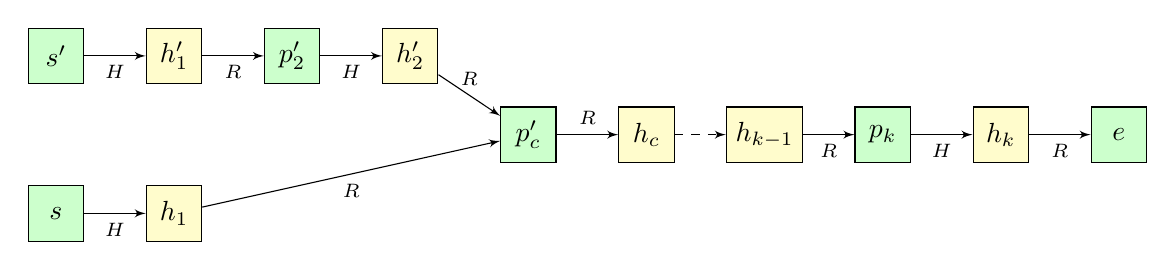
\begin{tikzpicture}[>=latex']

% Draw blocks, inputs and outputs

    \def\sp{1.5}
    \node[p] at (-2*\sp,-1) (hash0) {$s$};
    \node[p] at (7*\sp,0) (hash7) {$e$};
    \node[h] at (-1*\sp,-1) (hash1) {$h_1$};
    \node[h] at (3*\sp,0) (hash3) {$h_c$};
    \node[h] at (4*\sp,0) (hash4) {$h_{k-1}$};
    \node[p] at (5*\sp,0) (hash5) {$p_{k}$};
    \node[h] at (6*\sp,0) (hash6) {$h_{k}$};
    \draw[->] (hash0) -- node[below] {\scriptsize{$H$}} (hash1);
    \draw[->] (hash4) -- node[below] {\scriptsize{$R$}} (hash5);
    \draw[->] (hash5) -- node[below] {\scriptsize{$H$}} (hash6);
    \draw[->] (hash6) -- node[below] {\scriptsize{$R$}} (hash7);
    \draw[->, dashed] (hash3) -- (hash4);

    \node[p] at (-2*\sp,1) (hashs) {$s'$};
    \node[h] at (-1*\sp, 1) (hashp) {$h'_1$};
    \node[p] at (0*\sp, 1) (hashpa) {$p'_2$};
    \node[h] at (1*\sp, 1) (hashpa1) {$h'_2$};
    \node[p] at (2*\sp, 0) (hashpa2) {$p'_c$};
    \draw[->] (hash1) -- node[below] {\scriptsize{$R$}} (hashpa2);
    \node[] at (3*\sp, 1) (hashpb) {};
    \draw[->] (hashp) -- node[below]{\scriptsize{$R$}} (hashpa);
    \draw[->] (hashpa2) -- node[above]{\scriptsize{$R$}} (hash3);
    \draw[->] (hashs) -- node[below]{\scriptsize{$H$}} (hashp);
    \draw[->] (hashpa1) -- node[above]{\scriptsize{$R$}} (hashpa2);
    \draw[->] (hashpa) -- node[below]{\scriptsize{$H$}} (hashpa1);

\end{tikzpicture}
\end{center}
\caption{This is a demonstration of two chains colliding, from the point where $R$ is applied to $h'_2$ no more useful work is performed by the chain starting at $s'$.}
\label{fig:col}
\end{figure}

Selecting an appropriate reduction function is a critical part of the design of a hash-chain table. It is important to know a lot about the possible password domain as constraining the search to this area will be more useful and generating a smaller table while covering the likely password space with less gaps, increasing the chance of finding the hash and its inverse. It is also important to generate the correct distribution of messages, it may be inefficient to create many short passwords if the space is up to 9 character for example. Needless to say designing an appropriate reduction function is difficult.

\paragraph{Rainbow Tables}
The largest shortcoming of simple hash-chain tables is that the number of collisions increases as the table size increases. To overcome this in 2003 Oechslin\cite{Oechslin} proposed a method for using multiple reduction functions to drastically reduce the effect that a single collision has on the production of a chain in a table. This approach is called a rainbow table and is the dominant approach to launching pre-image attacks on hashing functions today.

A rainbow table has $k$ different reduction functions $R_1 \rightarrow R_k$ and these are applied sequentially, alternating between hash and reduction application as in the hash-chain approach. This greatly reduces the damage caused by a collision. Collisions will still occur as shown in figure \ref{fig:rain}, but in the next step the application of a different reduction function will diverge the two chains again. It is possible to still have a collision which wastes the chain: if both chains merge on the same step, this will tie the two chains in to exploring the same state-space. This is much rarer than the collision case in the simple hash-chain table.

Using a rainbow table is still quite simple, given a hash, $h$ to attack, the last reduction function, $R_k$ is applied and the table is searched for a chain which has a matching endpoint. This is an attempt at guessing that the hash was the last hash the table saw.
If none is found then the preceeding reduction $R_{k-1}$ is applied, followed by the hash and $R_k$. This is a guess that the $h$ was the penultimate hash seen in each table chain. This continues until a hit is found in the set of endpoints. Once it is the starting point is selected and the chain is replayed until $h$ is found, the preceeding password is the password which hashed to $h$, as with the hash-chain table.


The original rainbow table paper demonstration, by Oechslin, constructed a rainbow table and accompanying program to crack Windows passwords. The program and wider principle behind rainbow tables has been subsequently used to demonstrate the tractability of pre-image attacks given that distributed resources are now available. Projects including \texttt{freerainbowtables.com} use many clients to distribute the work of generating hash chains. These projects have created a wealth of tables which these writers believe, though they do not break the hash's cryptographic one-way nature, do undermine the security of existing hashes and should raise questions about the continued use of algorithms such as MD5 and SHA-1.

\begin{figure}
    \begin{center}
    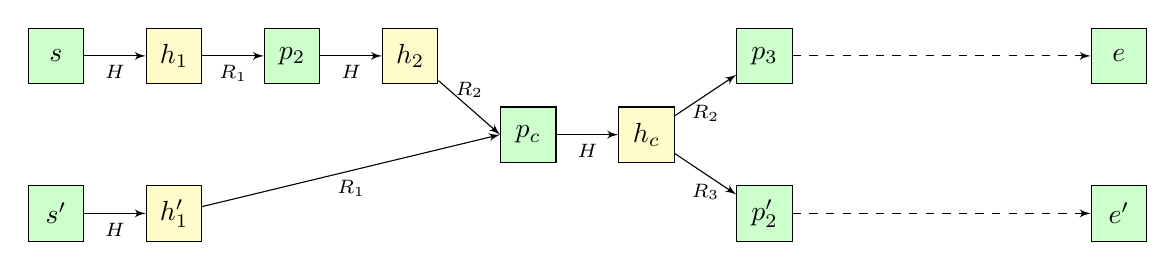
\begin{tikzpicture}[>=latex']

% Draw blocks, inputs and outputs

    \def\sp{1.5}
    \node[p] at (-2*\sp,1) (hash0) {$s$};
    \node[p] at (7*\sp,-1) (hashe1) {$e'$};
    \node[p] at (7*\sp,1) (hashe2) {$e$};
    \node[h] at (-1*\sp,1) (hash1) {$h_1$};
    \node[p] at (0*\sp,1) (hash2) {$p_2$};
    \node[h] at (1*\sp,1) (hash3) {$h_2$};
    \node[p] at (-2*\sp,-1) (hashs) {$s'$};
    \node[p] at (4*\sp,1) (hashb) {$p_3$};
    \node[p] at (4*\sp,-1)  (hashc) {$p'_2$};

    \node[h] at (-1*\sp, -1) (hashp) {$h'_1$};
    \node[p] at (2*\sp, 0) (hashpa2) {$p_c$};
    \node[] at (3*\sp, -1) (hashpb) {};
    \node[h] at (3*\sp,0) (hash6) {$h_c$};
    \draw[->] (hash0) -- node[below] {\scriptsize{$H$}} (hash1);
    \draw[->] (hash1) -- node[below] {\scriptsize{$R_1$}} (hash2);
    \draw[->] (hash2) -- node[below] {\scriptsize{$H$}} (hash3);
    \draw[->] (hash3) -- node[above] {\scriptsize{$R_2$}} (hashpa2.west);

    \draw[->] (hashp) -- node[below]{\scriptsize{$R_1$}} (hashpa2.west);
    \draw[->] (hashpa2) -- node[below]{\scriptsize{$H$}} (hash6);
    \draw[->] (hashs) -- node[below]{\scriptsize{$H$}} (hashp);
    \draw[->] (hash6) -- node[below] {\scriptsize{$R_2$}} (hashb);
    \draw[->] (hash6) -- node[below] {\scriptsize{$R_3$}} (hashc);
    \draw[->, dashed] (hashb) -- (hashe2);
    \draw[->, dashed] (hashc) -- (hashe1);

\end{tikzpicture}
\end{center}
\caption{In a rainbow table as there are several reduction functions, as they are applied sequentially any branches merging will likely split on the application of the different reduction function.}
\label{fig:rain}
\end{figure}

\subsection{Defending Against Tables}
Pre-image attacks using tables are extremely effective at cracking hashes for passwords in the their password domain, however protecting stored passwords against these tables is simple.

Instead of storing just the hash, $h$, of the password $p$ a salted hash is stored. Where $s$ is some fixed-known string (salt) a salted hash can simple be made by concatenating the hash and salt, $$h = H(p||s),$$ or $$h = H(H(p) || s).$$
The salt need not be kept a secret as it should not be of little help when attempting to calculate a pre-image. It is feasible to create a hash table which takes into account a salt, so using a single salt is not a particularly safe approach as a single hash table could release the passwords to an entire database. Usually a salted hash and the salt are stored together, but importantly a salt will be different for each password, possibly the timestamp of a sign-up time for example. Ensuring the individual salts are different ensures that a fresh table would have to be created to crack each password and reduces any attack to a brute force approach, which is the best case.

An alternative defence would be to make the construction of such a table inconceivable. This can be achieved by a process called key-strectching. This process repeatedly applies the hashing function (often in excess of 1000) times to the password, this has the effect of increasing the amount of time it takes to compute each hash in the chain. This has a drastic impact on the total time taken to produce the table.This approach is susceptable to a very specific type of attack, one using custom hardware. 
Using FPGAs it is possible to construct hardware circuit which are able to unroll these repetition loops and therefore circumvent the added complexity added by the repetition stretching, this is a very specialised attack however and only viable when a lot of information is known about the encryption system. The custom hardware necessary would be very expensive and approaches such as \textbf{scrypt}\cite{colin} which as part of their process deliberately inflate memory usage have been futher developed to make specialist hardware and parallelism a less viable option for producing large amounts of hashes.



\section{Side Channel Attacks}
A side channel attack is an attack on the physical implementation of the cryptosystem. The main attacks are based on the fact there are effecient ways to do certain mathmatical functions on a processor based on the values being processed, this is usually branching dependent on whether particular bits are 0 or 1. This approach has been widely applied on 3-DES schemes and only tried occasionally, with limited success to traditional hashes, such as MD5.

\subsection{Power Attacks}
There are two types of Power Attacks. Using Simple Power Analysis(SPA) is simply watching the trace of the power flowing through the processer while it is performing the functions this shows the load on the processer and from that work out what action is being done. Peter Kocher outlined using DES in \cite{kocherPower} showing that you can see the distinct rounds in the DES structure. 

\begin{figure}
    \includegraphics[width=\textwidth]{SPAtrace.png}
    \caption{Trace showing a SPA of an entire DES operation.}
    \label{fig:desRound}
\end{figure}
The other type is a Differential Power Analysis where many different checks are used and then a difference is applied to only show the `significant' changes. Looking at DES in a round of the encryption the 8 S-Boxes each take 6 subkey bits and 6 bits of the R side and produce 4 bits of output as described in \cite{otherPaper}. The selection function $D(C,b,K_s)$ is defined as the value of the bit $0 \le b < 32$ of the DES L side before working out the 16th round for the cipher text $C$, where the 6 key bits entering the S box corresponding to the bit $b$ are $0 \le K_s < 2^6$. If we have the wrong key bits we will get the bit $b$ right half of the time due to chance. 

To use the DPA attack first takes $m$ samples of cipher text and power traces $T_{1..m}[1..k]$ containing $k$ samples each and evaluates $D$ for them and seperates them into two groups $g_0$ and $g_1$ where the evaluations for $b$ are 0 and 1 respectivly. Then $\Delta_D$ is worked out for the means of the traces from $g_0$ and $g_1$. Then $\Delta_D[j]$ is the average over $C_{1..m}$ of the change due to the value of the selection function $D$ on the power consumption at point $j$. 
\begin{align}
    \Delta_D[j] &= \frac{\sum_{i=1}^mD(C_i,b,K_s)T_i[j]}{\sum_{i=1}^mD(C_i,b,K_s)} -  \frac{\sum_{i=1}^m(1-D(C_i,b,K_s))T_i[j]}{\sum_{i=1}^m(1-D(C_i,b,K_s))}\\
    &\approx 2( \frac{\sum_{i=1}^mD(C_i,b,K_s)T_i[j]}{\sum_{i=1}^mD(C_i,b,K_s)} - \frac{\sum_{i=1}^mT_i[j]}{m}) 
\end{align}

If $K_s$ is correct however, the calulation of $D$ will be correct for all the cipher text. As a result the $\Delta_D[j]$ will approach the effect of the target bit on the power consumption as $m \rightarrow \infty$.

The correct value of $K_s$ can be identified from the spikes in the differential traces. Four values of $b$ correspond to each S Box, providing validation of key block guesses. If you find all the eight $K_s$ gives you the entire 48-bit round subkey. The remaining 8 key bits can be found either by exhaustive search or the attack could be focused on another round of the DES sequence. Triple DES keys can be found by analyzing the outer DES operation, finding the key to decrypt the ciphertext and then attacking the next DES key. Shown in figure~\ref{fig:desResult} are 4 traces of a reference trace followed by correct $K_s$ and two incorrect one.

\begin{figure}
    \includegraphics[width=\textwidth]{DPATraces.png}
    \caption{Traces showing the average trace then one with a correct guess of $K_s$ and the bottom two with incorrect guesses with $m = 1000$}
    \label{fig:desResult}
\end{figure}


There is the belief that using there is a possibility to use DPA on a HMAC-MD5 based on a smartcard, due to the ease of control timing cycles and power input. This is outlined in \cite{JiriKur}. However this turns out to be false and is blamed on the equipment used as this was set up with standard equipment not specialist equipment, it is suggested specialist hardware could improve the results. This would suggest, at the current time, that this type of attack best suited for to attacks on DES or RSA as described above.

\subsection{Timing Attacks}
There are quite a few different types of timing attacks which essentially take advantage of algorithms taking shortcuts to save computing power based on what it is processing. One of which is for computing $R = y^x \mod n$, where $x$ is $w$ bits long, which is used in RSA, is shown in~\ref{alg:expSquare} where $X_k$ means the $k^{th}$ bit of $x$ as you can see if the bit of the exponent is 1 we have to compute an extra muliplication step which gives us the possibility of watching out for how long a pass through the algorithm takes which would give us if $X_k$ is 0 or 1, which means we can rebuild the exponent. This is critical in RSA as $y$ is the cipher text which can be easvedropped upon and $n$ is public. This is outlined in \cite{crosbyTiming} as a possibility to crack RSA over the internet based on large number of observations to counteract the noise of the timing data.

Another type of timing attack is due to how checks of equality of iterables are usually lazily evaluated, as in they cut out when they find they are inequal as there is no gain from finishing the comparison due to no additional information gained. This has lead to the ability to see \emph{how many bits we got right} \cite{lessonInTiming} this shows how problems can occur essentially outside of how secure any crypto algorithm is if there is side channel leak of information due to implementation either in the hardware running it or the exact way programmatically the algorithm is implemented.


\begin{algorithm}
    \caption{Exponentiation By Squaring based off of the explination in \cite{kocherTiming}}
    \label{alg:expSquare}
\begin{algorithmic}
    \State $S_0 \gets 1$
    \For{$k = 0 \to w - 1 $}
    \If{$X_k = 1$}
        \State $R_k \gets (s_k * y) \mod n$
    \Else
        \State $R_k \gets s_k$
    \EndIf
    \State $s_{k+1} \gets R_k^2 \mod n$
    \EndFor\\
    \Return $(R_{w-1})$
\end{algorithmic}
\end{algorithm}

\bibliography{library}
\bibliographystyle{plain}

Resources:

MIT Crypto lectures: http://cseweb.ucsd.edu/~mihir/papers/gb.pdf
A Lesson In Timing Attacks: http://codahale.com/a-lesson-in-timing-attacks/
Timing Attacks on Implementations of Diffie-Hellman, RSA, DSS, and Other Systems, P. Kocher.: http://www.cryptography.com/public/pdf/TimingAttacks.pdf
Differential Power Analysis: http://www.cryptography.com/public/pdf/DPA.pdf
Algorithms for differential power analysis of the cryptographic smart cards: https://is.muni.cz/th/98692/fi\_b/bc\_thesis\_Jiri\_Kur.pdf
Merkle thesis: http://www.merkle.com/papers/Thesis1979.pdf 
MD5 spec: http://tools.ietf.org/html/rfc1321 
@misc{cryptoeprint:2004:199,
    author = {Xiaoyun Wang  and Dengguo Feng and Xuejia Lai and Hongbo Yu},
    title = {Collisions for Hash Functions MD4, MD5, HAVAL-128 and RIPEMD},
    howpublished = {Cryptology ePrint Archive, Report 2004/199},
    year = {2004},
%    note = {\url{http://eprint.iacr.org/}},
}

\lstinputlisting[language=Python]{../md5.py}

\end{document}
